\documentclass[10pt,a4paper,openany,twoside, eleve]{book}

\usepackage{layout_cours}
\setlist{leftmargin=5mm}

\begin{document}
	\chapnumber{8} % numéro du chapitre
	\titre{Etude du sens de variation d'une fonction} % titre du chapitre
	\classe{Seconde} % classe
	\entetegal

	% Debut du texte
	% **************

	\vspace{-7mm}
	\paragraph*{Objectif du chapitre :}
	\begin{itemize}  
		\vspace{-2mm}
		\setlength\itemsep{-1mm}
		\item Déterminer, à partir de la courbe représentative, le sens de variation de la fonction et le tableau de variation de la fonction.
		\item A partir du tableaux de variation, comparer deux images par une fonction et déterminer les extremums d'une fonction.
	\end{itemize}
	\vspace{-7mm}
	
	\section{Sens de variation}
	
	\begin{defi}{Sens de variation}{}
	\begin{enumerate}
		\item On dit que la fonction $f$ est \textbf{strictement croissante} sur un intervalle $I$ si pour tous $a, b \in I$ tels que $a < b$, on a $f(a) < f(b)$. \\ 
		Autrement dit, les images de $a$ et de $b$ sont rangées dans le même ordre que $a$ et $b$.
		\item 
		On dit que la fonction $f$ est \textbf{strictement décroissante} sur un intervalle $I$ si pour tous $a, b \in I$ tels que $a < b$, on a $f(a) > f(b)$. \\ 
		Autrement dit, les images de $a$ et de $b$ sont rangées dans l'ordre inverse de $a$ et $b$.
		\item  On dit que la fonction $f$ est \textbf{constante} sur un intervalle $I$ si pour tous $a, b \in I$, on a $f(a) = f(b)$. \\ 
	\end{enumerate}
	\begin{multicols}{2}
	\begin{center}
	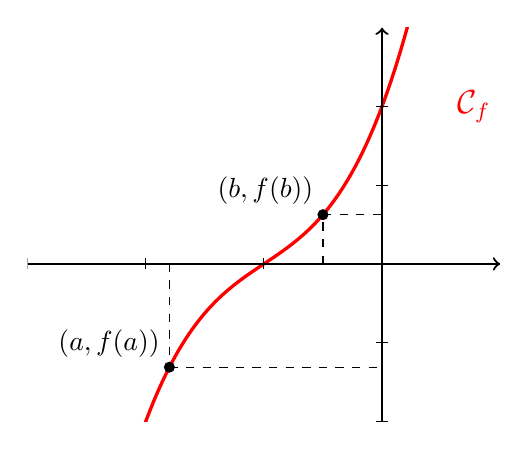
\begin{tikzpicture}[x=1.5cm]
		%Fonction	
		\clip(-3,-2) rectangle (1,3);
		\draw[line width=1.2pt,color=red,smooth,samples=100,domain=-3:1] plot(\x,{(\x+1)^(3.0)+1+\x})node [right] {\large{$\mathcal{C}_{f}$}};       
		\draw[red] (1,2) node[left] {\large{$\mathcal{C}_{f}$}};
		
		% Axes
		\draw[thick,->] (-3,0) -- (1,0);
		\draw[thick,->] (0,-2) -- (0,3);

		\foreach \x in {-3,-2,-1}
			\draw[shift={(\x,0)},color=black] (0pt,2pt) -- (0pt,-2pt);
		\foreach \y in {-2,-1,1,2}
			\draw[shift={(0,\y)},color=black] (2pt,0pt) -- (-2pt,-0pt);

		% Calculate the function values at x = -1.8 and x = -0.5
		\pgfmathsetmacro\a{(-1.8+1)^3 + 1-1.8}
		\pgfmathsetmacro\b{(-0.5+1)^3 + 1-0.5}
	
		% Draw dashed lines from the curve to the x-axis (at x = -1.8 and x = -0.5)
		\draw[dashed] (-1.8,0) -- (-1.8,\a);
		\draw[dashed] (-0.5,0) -- (-0.5,\b);
	
		% Draw horizontal lines at y = f(a) and y = f(b)
		\draw[dashed] (-1.8,\a) -- (0,\a);  % Horizontal line at f(a)
		\draw[dashed] (-0.5,\b) -- (0,\b);  % Horizontal line at f(b)
	
		% Add points on the curve
		\fill (-1.8,\a) circle (2pt);
		\fill (-0.5,\b) circle (2pt);
	
		% Add labels for the points
		\node[above left] at (-1.8,\a) {$(a, f(a))$};
		\node[above left] at (-0.5,\b) {$(b, f(b))$};
		
		\end{tikzpicture}\\
		fonction strictement croissante
	\end{center}
	\begin{center}
	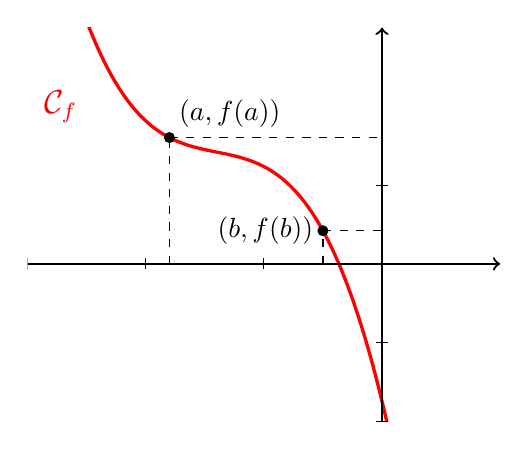
\begin{tikzpicture}[x=1.5cm]
		%Fonction	
		\clip(-3,-2) rectangle (1,3);
		\draw[line width=1.2pt,color=red,smooth,samples=100,domain=-3:1] plot(\x,{-(\x+1.4)^(3.0)+1-0.3*\x});       
		\draw[red] (-2.5, 2) node[left] {\large{$\mathcal{C}_{f}$}};
		
		% Axes
		\draw[thick,->] (-3,0) -- (1,0);
		\draw[thick,->] (0,-2) -- (0,3);
		\foreach \x in {-3,-2,-1}
			\draw[shift={(\x,0)},color=black] (0pt,2pt) -- (0pt,-2pt);
		\foreach \y in {-3,-2,-1,1}
			\draw[shift={(0,\y)},color=black] (2pt,0pt) -- (-2pt,-0pt);
		
		% Calculate the function values at x = -1.8 and x = -0.5
		\pgfmathsetmacro\a{-(-1.8+1.4)^3 + 1 + 0.3*1.8}
		\pgfmathsetmacro\b{-(-0.5+1.4)^3 + 1 + 0.3*0.5}
	
		% Draw dashed lines from the curve to the x-axis (at x = -1.8 and x = -0.5)
		\draw[dashed] (-1.8,0) -- (-1.8,\a);
		\draw[dashed] (-0.5,0) -- (-0.5,\b);
	
		% Draw horizontal lines at y = f(a) and y = f(b)
		\draw[dashed] (-1.8,\a) -- (0,\a);  % Horizontal line at f(a)
		\draw[dashed] (-0.5,\b) -- (0,\b);  % Horizontal line at f(b)
	
		% Add points on the curve
		\fill (-1.8,\a) circle (2pt);
		\fill (-0.5,\b) circle (2pt);
	
		% Add labels for the points
		\node[above right] at (-1.8,\a) {$(a, f(a))$};
		\node[ left] at (-0.5,\b) {$(b, f(b))$};

	\end{tikzpicture}\\
	fonction strictement décroissante
	\end{center}
	\end{multicols}
\end{defi}
	
\begin{rem}{}{}
	Le sens de variation dépend de l'intervalle $I$ considéré. 
	Donner les variations d'une fonction signifie préciser sur quels intervalles la fonction est strictement croissante, strictement décroissante ou constante.
	
\end{rem}
	
	\begin{ex}{}{}
		\label{ex1}
		\begin{minipage}{0.5\textwidth}
			Dans cet exemple, on se contente de décrire graphiquement ce que l'on observe sans rien démontrer formellement.\medskip
			\newline
			Graphiquement, cette fonction semble \textcolor{purple}{strictement décroissante sur $[-4,-2.1]$}, \textcolor{blue}{strictment croissante sur $[-2.1,0]$}, \textcolor{purple}{strictement décroissante sur $[0,4.1]$}, \textcolor{blue}{puis strictement croissante sur $[4.1,5]$}.
			\medskip
			\newline
			Les valeurs de la fonction $f$ à ces abscisses serviront à dresser le tableau de variation.
			\begin{align*}
				f(-4) &= 11\\
				f(-2.1) &= 4\\
				f(0) &= 5\\
				f(4.1) &= -3.7\\
				f(5) &= -2\\
			\end{align*}
		\end{minipage}
		\hspace{5mm}
		\begin{minipage}{0.5\textwidth}
			\begin{center}
				\begin{tikzpicture}[line cap=round,line join=round,>=triangle 45,x=0.9cm,y=0.375cm,scale=0.9]
					%Fonction	
					\draw[line width=1.2pt,color=purple,smooth,samples=100,domain=-4:-2.1] plot(\x,{0.0385*(\x)^(4.0)-0.1*(\x)^(3.0)-0.7*(\x)^(2.0)-0.15*(\x)+5.0});   
					\draw[line width=1.2pt,color=blue,smooth,samples=100,domain=-2.1:0] plot(\x,{0.0385*(\x)^(4.0)-0.1*(\x)^(3.0)-0.7*(\x)^(2.0)-0.15*(\x)+5.0});
					\draw[line width=1.2pt,color=purple,smooth,samples=100,domain=0:4.1] plot(\x,{0.0385*(\x)^(4.0)-0.1*(\x)^(3.0)-0.7*(\x)^(2.0)-0.15*(\x)+5.0});
					\draw[line width=1.2pt,color=blue,smooth,samples=100,domain=4.1:5] plot(\x,{0.0385*(\x)^(4.0)-0.1*(\x)^(3.0)-0.7*(\x)^(2.0)-0.15*(\x)+5.0})node [right] {\large{$\mathcal{C}_{f}$}};
					\draw[line width=1pt,dashed] (-2.1,0) -- (-2.1,4);
					\draw[line width=1pt,dashed] (-2.1,4) -- (0,4);
					\draw[line width=1pt,dashed] (4.1,0) -- (4.1,-3);
					\draw[line width=1pt,dashed] (4.1,-3.5) -- (0,-3.5);
					\draw[line width=1pt,dashed] (-4,0) -- (-4,11);
					\draw[line width=1pt,dashed] (-4,11) -- (0,11);
					% Axes
					\draw[thick,->] (-4.5,0) -- (5.5,0);
					\foreach \x in {-4,-3,-2,-1,1,2,3,4,5}
					\draw[shift={(\x,0)},color=black] (0pt,2pt) -- (0pt,-2pt)node[below] {\footnotesize $\x$};
					\draw[thick,->] (0,-4) -- (0,13);
					\foreach \y in {-4,-2,2,4,6,8,10,12}
					\draw[shift={(0,\y)},color=black] (2pt,0pt) -- (-2pt,-0pt)node[left] {\footnotesize $\y$};
				\end{tikzpicture}\\
			\end{center}
		\end{minipage}
	\vspace{-8mm}
	\end{ex}

\begin{defi}{Sens de variation au sens large}{}
	On dit que la fonction $f$ est \textbf{croissante au sens large} (ou simplement croissante) sur un intervalle $I$ si pour tous $a, b \in I$ tels que $a < b$, on a $f(a) \le f(b)$. \\ 
	On dit que la fonction $f$ est \textbf{décroissante} (ou simplement décroissante) sur un intervalle $I$ si pour tous $a, b \in I$ tels que $a < b$, on a $f(a) \ge f(b)$. \\ 

	\vspace{3mm}
	De manière équivalente : 

	On dit que la fonction $f$ est \textbf{croissante au sens large} sur un intervalle $I$, si on peut découper l'intervalle $I$ en une union $I = J_1 \cup J_2 \cup ... \cup J_n \cup K_1 \cup K_2 \cup ... \cup K_m$ tels que $f$ est strictement croissante sur $J_1, J_2, ..., J_n$ et constante sur $K_1, K_2, ..., K_m$. \\ 
	On dit que la fonction $f$ est \textbf{décroissante au sens large} sur un intervalle $I$, si on peut découper l'intervalle $I$ en une union $I = J_1 \cup J_2 \cup ... \cup J_n \cup K_1 \cup K_2 \cup ... \cup K_m$ tels que $f$ est strictement décroissante sur $J_1, J_2, ..., J_n$ et constante sur $K_1, K_2, ..., K_m$. \\ 
\end{defi}

\begin{ex}{}{}
	
	On peut découper l'intervalle $I = \ff{-3}{1}$:
	\vspace{1mm}
	$I = J_1 \cup K_1 \cup J_2 = \ff{-3}{-1} \cup \ff{-1}{0} \cup \ff{0}{1}$
	
	\begin{itemize}
		\item 
		$f$ est strictement croissante sur $J_1=\ff{-3}{-1}$ et $J_2 = \ff{0}{1}$.
		\item 
		$f$ est constante sur $K_1=\ff{-1}{0}$.
	\end{itemize}
	Donc la fonction $f$ ci-dessous est croissante au sens large sur l'intervalle $I= \ff{-3}{1}$.
\begin{center}
	\begin{tikzpicture}[x=1.5cm]
		%Fonction	
		\clip(-3,-2) rectangle (1.5,3);
		\draw[line width=1.2pt,color=red,smooth,samples=100,domain=-3:-1] plot(\x,{3*(\x+1)^(3.0)++1});       
		\draw[line width=1.2pt,color=red,smooth,samples=100,domain=0:1] plot(\x,{3*(\x)^(3.0)+1});       
		\draw[line width=1.2pt,color=red,smooth,samples=100,domain=-1:0] plot(\x,{1});       
		\draw[red] (1,1.5) node {\large{$\mathcal{C}_{f}$}};
		
		% Axes
		\draw[thick,->] (-3,0) -- (1,0);
		\draw[thick,->] (0,-2) -- (0,3);

		\foreach \x in {-3,-2,-1,1}{
			\draw[shift={(\x,0)},color=black] (0pt,2pt) -- (0pt,-2pt);
			\node[below] at (\x, 0) {\x};
			}
		\foreach \y in {-2,-1,1,2}{

			\draw[shift={(0,\y)},color=black] (2pt,0pt) -- (-2pt,-0pt);
			}
		\end{tikzpicture}\\
	\end{center}
\end{ex}

	\section{Tableau de variation}
	
	\begin{defi}{Tableau de variation}{}
		Le \textbf{tableau de variation} d'une fonction est un tableau synthétique regroupant les informations concernant les variations de la fonction.
	\end{defi}

	\begin{ex}{}{}
	Le tableau de variation de la fonction $f$ de l'exemple \ref{ex1} est :
	\begin{center}
		\begin{tikzpicture}
			\tkzTabInit{$x$/1,$f$/2}
			{$-4$,$-2.1$,$0$,$4.1$,$5$}
			%\tkzTabLine{t,+,z,-,t}
			\tkzTabVar{+/$11$,-/$4$,+/$5$,-/$-3.7$,+/$-2$}
			\end{tikzpicture}
		\end{center}
	\end{ex}
	
	\begin{rem}{}{}
		Sauf indication contraire, les flèches désignent une croissance ou une décroissance \textbf{stricte}. 
	\end{rem}

	\begin{methode}{Tracer l'allure d'une courbe à partir du tableau de variation}{}
		\begin{enumerate}
			\item On commence par placer les points particuliers.
			\item A main levée, on trace une courbe qui passe par ces points. On vérifie bien que la courbe respecte les variations du tableau (croissance ou décroissance).
			
			Généralement les fonctions étudiées sont régulières. Donc on peut essayer de faire une courbe lissée.
		\end{enumerate}

		\begin{center}
			\begin{tikzpicture}
				\tkzTabInit{$x$/1,$f$/2}
				{$-4$,$-1$,$0$,$2$}
				%\tkzTabLine{t,+,z,-,t}
				\tkzTabVar{+/$-1$,-/$-2$,+/$1$,-/$-3$}
			\end{tikzpicture}

			\vspace{10mm}
			
			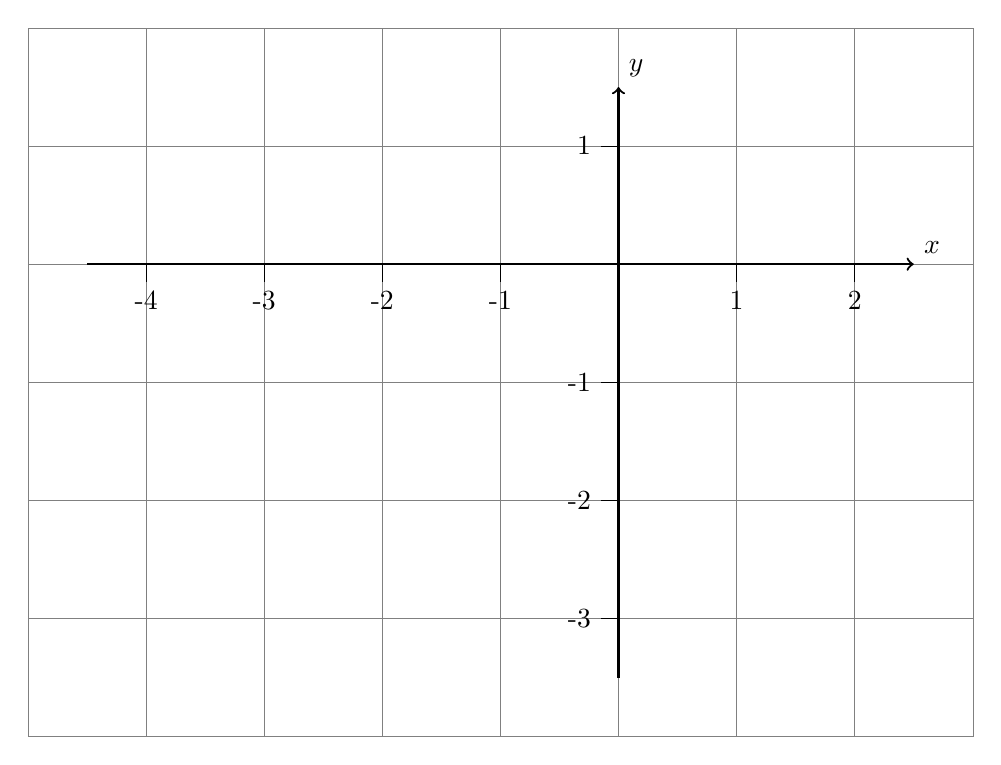
\begin{tikzpicture}[scale=1.5]
				% Draw grid
				\draw[step=1cm,gray,very thin] (-5,-4) grid (3,2);
			
				% Draw axes
				\draw[thick,->] (-4.5,0) -- (2.5,0) node[above right] {$x$};
				\draw[thick,->] (0,-3.5) -- (0,1.5) node[above right] {$y$};
			
				% Add automatic ticks on x-axis
				\foreach \x in {-4,-3,-2,-1,1,2}
					\draw (\x,0) -- (\x,-0.15) node[below] {\x};
			
				% Add automatic ticks on y-axis
				\foreach \y in {-3,-2,-1,1}
					\draw (0,\y) -- (-0.15,\y) node[left] {\y};
			\end{tikzpicture}
		\end{center}

	\end{methode}

	\newpage

	\section{Sens de variation et inéquation}

	\begin{prop}{Sens de variation d'une fonction affine}{var_fonction_affine}
		Soit $\alpha,\beta\in\R$. Soit $\fonction{f}{\R}{\R}{x}{\alpha x+\beta}$.

		\begin{itemize}
			\item Si $\alpha >0$, alors $f$ est strictement croissante.
			\item Si $\alpha =0$, alors $f$ est constante.
			\item Si $\alpha <0$, alors $f$ est strictement décroissante.
		\end{itemize}
	\end{prop}

	\begin{dem}{}{}
		\dotsfill{15}
	\end{dem}

	\begin{rem}{}{}
		La propriété \ref{propo:var_fonction_affine} est équivalente aux règles de calcul des inéquations.

		Par exemple, on sait que multiplier par un nombre $\alpha<0$ négatif modifie le sens de l'inégalité:
		\begin{align*}
			a<b 
			\quad \implies \quad \alpha * a > \alpha * b 
		\end{align*}

		Soit $f:x\longmapsto \alpha x$. Alors $f$ est décroissante d'après la propriété \ref{propo:var_fonction_affine}. et on peut réécrire l'inégalité:
		\begin{align*}
			a<b 
			\quad \implies \quad f(a) > f(b) 
		\end{align*}
	
	\end{rem}

	\section{Extremum}
	
	\begin{defi}{Minimum}{}
	On dit que la fonction $f$ admet un \textbf{minimum} $m$ sur un intervalle $I$, atteint en $x_0$ si, quel que soit le réel $x$ dans $I$, on a $f(x) \ge f(x_0)=m$.
	\end{defi}
	
	\begin{defi}{Maximum}{}
	On dit que la fonction $f$ admet un \textbf{maximum} $M$ sur un intervalle $I$, atteint en $x_0$ si, quel que soit le réel $x$ dans $I$, on a $f(x) \le f(x_0)=M$.
	\end{defi}
	
	\begin{rem}{}{}
		Un \bf{extremum} est soit un minimum soit un maximum.

		Les mots extremum, minimum et maximum proviennent du latin. Les mots pluriels sont \emph{extrema}, \emph{minima} et \emph{maxima} 
	\end{rem}
	\begin{ex}{}{}
		Pour la fonction $f$ de l'exemple \ref{ex1} : 
		\begin{itemize}
			\item  Le maximum sur $[-4;5]$ est $M=11$, atteint pour $x=-4$.
			\item  Le minimum sur $[-4;5]$ est $m=-3,5$, atteint pour $x=4,1$.
		\end{itemize}
	\end{ex}
	
	\begin{rem}{}{}
		La valeur d'un extremum dépend de l'intervalle !\\
		Pour la fonction $f$ de l'exemple \ref{ex1}, le maximum sur $[-2;4]$ est $M=5$, atteint pour $x=0$.
	\end{rem}

	\section{Exercices}
	\begin{exercices}
		\sectionexo{Sens de variation}
	\begin{bookexo}{56 p.254}\end{bookexo}
	\begin{bookexo}{54 p.254}\end{bookexo}
	\begin{bookexo}{44 p.252}\end{bookexo}
	\begin{bookexo}{46 p.252}\end{bookexo}
	\sectionexo{Tableau de variation}
	\begin{bookexo}{58 p.254}\end{bookexo}
	\begin{bookexo}{60 p.255}\end{bookexo}
	\sectionexo{Tracé de courbe à partir du tableau de variations}
	\begin{bookexos}{49,50 p.253}\end{bookexos}
	\sectionexo{Fonction affine}
	\begin{bookexo}{69 p.256}\end{bookexo}
	\begin{bookexo}{72 p.257}\end{bookexo}
	\begin{bookexo}{74 p.257}\end{bookexo}
	\sectionexo{Extremum}
	\begin{bookexo}{55 p.254}\end{bookexo}
	\begin{bookexo}{64 p.255}\end{bookexo}
	\sectionexo{Transversal}
	\begin{bookexo}{62 p.255}\end{bookexo}
	\end{exercices}
	% \section{Tableau de signes}
	
	% On réunit au sein d'un tableau appelé \textbf{tableau de signes} les informations concernant le signe de la fonction $f$, c'est à dire sa position par rapport à l'axe des abscisses
	
	% \begin{ex}{}{}
	% Le tableau de signe de la fonction $f$ est :
	% \begin{center}
	% \begin{tikzpicture}
	% \tkzTabInit{$x$/1,$f(x)$/1}
	% {$-4$,$2.5$,$5$}
	% \tkzTabLine{t,+,z,-,t}
	% %\tkzTabVar{+/$+\infty$,-/$0$,+/$+\infty$}
	% \end{tikzpicture}
	% \end{center}
	% \end{ex}
	
	% \begin{methode}{Etablir le tableau de signes de $f$ définie sur $\R$}{}
	% 	\begin{itemize}
	% 		\item A partir du graphe de la fonction, je peux étudier le signe. Lorsque le graphe est en dessous de l'axe des abscisses, alors $f(x)\le 0$. Lorsque le graphe est au dessus, $f(x)\ge 0$.
	% 		\item Je résous l'équation $f(x)=0$. Par exemple, les solutions sont $x_1\in\R$ et $x_2\in\R$, avec $x_1 < x_2$. Alors j'étudie $f$ sur les intervalles suivants: $\oo{-\infty}{x_1}$, $\oo{x_1}{x_2}$, et $\oo{x_2}{+\infty}$,
	% 	\end{itemize}
	% \end{methode}
	
	%**************
	% Fin du texte

\end{document}

